% Created by tikzDevice version 0.10.1 on 2017-11-29 19:14:35
% !TEX encoding = UTF-8 Unicode
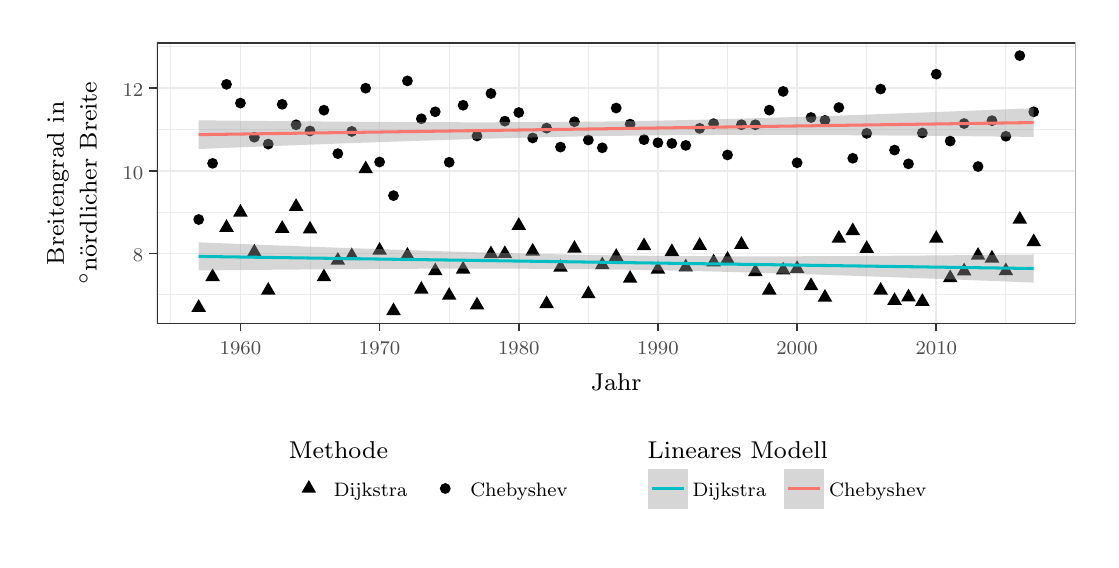
\begin{tikzpicture}[font=\footnotesize,x=1pt,y=1pt]
\definecolor{fillColor}{RGB}{255,255,255}
\path[use as bounding box,fill=fillColor,fill opacity=0.00] (0,0) rectangle (384.11,184.94);
\begin{scope}
\path[clip] (  0.00,  0.00) rectangle (384.11,184.94);
\definecolor{drawColor}{RGB}{255,255,255}
\definecolor{fillColor}{RGB}{255,255,255}

\path[draw=drawColor,line width= 0.6pt,line join=round,line cap=round,fill=fillColor] (  0.00,  0.00) rectangle (384.11,184.94);
\end{scope}
\begin{scope}
\path[clip] ( 46.70, 77.99) rectangle (378.61,179.44);
\definecolor{fillColor}{RGB}{255,255,255}

\path[fill=fillColor] ( 46.70, 77.99) rectangle (378.61,179.44);
\definecolor{drawColor}{gray}{0.92}

\path[draw=drawColor,line width= 0.3pt,line join=round] ( 46.70, 88.46) --
	(378.61, 88.46);

\path[draw=drawColor,line width= 0.3pt,line join=round] ( 46.70,118.31) --
	(378.61,118.31);

\path[draw=drawColor,line width= 0.3pt,line join=round] ( 46.70,148.16) --
	(378.61,148.16);

\path[draw=drawColor,line width= 0.3pt,line join=round] ( 46.70,178.01) --
	(378.61,178.01);

\path[draw=drawColor,line width= 0.3pt,line join=round] ( 51.73, 77.99) --
	( 51.73,179.44);

\path[draw=drawColor,line width= 0.3pt,line join=round] (102.02, 77.99) --
	(102.02,179.44);

\path[draw=drawColor,line width= 0.3pt,line join=round] (152.31, 77.99) --
	(152.31,179.44);

\path[draw=drawColor,line width= 0.3pt,line join=round] (202.60, 77.99) --
	(202.60,179.44);

\path[draw=drawColor,line width= 0.3pt,line join=round] (252.89, 77.99) --
	(252.89,179.44);

\path[draw=drawColor,line width= 0.3pt,line join=round] (303.18, 77.99) --
	(303.18,179.44);

\path[draw=drawColor,line width= 0.3pt,line join=round] (353.47, 77.99) --
	(353.47,179.44);

\path[draw=drawColor,line width= 0.3pt,line join=round] (378.61, 77.99) --
	(378.61,179.44);

\path[draw=drawColor,line width= 0.6pt,line join=round] ( 46.70,103.39) --
	(378.61,103.39);

\path[draw=drawColor,line width= 0.6pt,line join=round] ( 46.70,133.24) --
	(378.61,133.24);

\path[draw=drawColor,line width= 0.6pt,line join=round] ( 46.70,163.09) --
	(378.61,163.09);

\path[draw=drawColor,line width= 0.6pt,line join=round] ( 76.88, 77.99) --
	( 76.88,179.44);

\path[draw=drawColor,line width= 0.6pt,line join=round] (127.17, 77.99) --
	(127.17,179.44);

\path[draw=drawColor,line width= 0.6pt,line join=round] (177.46, 77.99) --
	(177.46,179.44);

\path[draw=drawColor,line width= 0.6pt,line join=round] (227.74, 77.99) --
	(227.74,179.44);

\path[draw=drawColor,line width= 0.6pt,line join=round] (278.03, 77.99) --
	(278.03,179.44);

\path[draw=drawColor,line width= 0.6pt,line join=round] (328.32, 77.99) --
	(328.32,179.44);
\definecolor{fillColor}{RGB}{0,0,0}

\path[fill=fillColor] ( 61.79,115.62) circle (  1.96);

\path[fill=fillColor] ( 66.82,135.92) circle (  1.96);

\path[fill=fillColor] ( 71.85,164.46) circle (  1.96);

\path[fill=fillColor] ( 76.88,157.69) circle (  1.96);

\path[fill=fillColor] ( 81.91,145.36) circle (  1.96);

\path[fill=fillColor] ( 86.93,142.87) circle (  1.96);

\path[fill=fillColor] ( 91.96,157.24) circle (  1.96);

\path[fill=fillColor] ( 96.99,149.84) circle (  1.96);

\path[fill=fillColor] (102.02,147.61) circle (  1.96);

\path[fill=fillColor] (107.05,155.11) circle (  1.96);

\path[fill=fillColor] (112.08,139.42) circle (  1.96);

\path[fill=fillColor] (117.11,147.44) circle (  1.96);

\path[fill=fillColor] (122.14,163.06) circle (  1.96);

\path[fill=fillColor] (127.17,136.40) circle (  1.96);

\path[fill=fillColor] (132.19,124.25) circle (  1.96);

\path[fill=fillColor] (137.22,165.71) circle (  1.96);

\path[fill=fillColor] (142.25,152.02) circle (  1.96);

\path[fill=fillColor] (147.28,154.55) circle (  1.96);

\path[fill=fillColor] (152.31,136.31) circle (  1.96);

\path[fill=fillColor] (157.34,156.90) circle (  1.96);

\path[fill=fillColor] (162.37,145.80) circle (  1.96);

\path[fill=fillColor] (167.40,161.16) circle (  1.96);

\path[fill=fillColor] (172.43,151.15) circle (  1.96);

\path[fill=fillColor] (177.46,154.28) circle (  1.96);

\path[fill=fillColor] (182.48,145.08) circle (  1.96);

\path[fill=fillColor] (187.51,148.64) circle (  1.96);

\path[fill=fillColor] (192.54,141.79) circle (  1.96);

\path[fill=fillColor] (197.57,150.94) circle (  1.96);

\path[fill=fillColor] (202.60,144.35) circle (  1.96);

\path[fill=fillColor] (207.63,141.52) circle (  1.96);

\path[fill=fillColor] (212.66,155.90) circle (  1.96);

\path[fill=fillColor] (217.69,150.08) circle (  1.96);

\path[fill=fillColor] (222.72,144.46) circle (  1.96);

\path[fill=fillColor] (227.74,143.36) circle (  1.96);

\path[fill=fillColor] (232.77,143.11) circle (  1.96);

\path[fill=fillColor] (237.80,142.40) circle (  1.96);

\path[fill=fillColor] (242.83,148.54) circle (  1.96);

\path[fill=fillColor] (247.86,150.26) circle (  1.96);

\path[fill=fillColor] (252.89,138.95) circle (  1.96);

\path[fill=fillColor] (257.92,149.88) circle (  1.96);

\path[fill=fillColor] (262.95,149.85) circle (  1.96);

\path[fill=fillColor] (267.98,155.15) circle (  1.96);

\path[fill=fillColor] (273.00,161.90) circle (  1.96);

\path[fill=fillColor] (278.03,136.13) circle (  1.96);

\path[fill=fillColor] (283.06,152.47) circle (  1.96);

\path[fill=fillColor] (288.09,151.44) circle (  1.96);

\path[fill=fillColor] (293.12,156.07) circle (  1.96);

\path[fill=fillColor] (298.15,137.74) circle (  1.96);

\path[fill=fillColor] (303.18,146.74) circle (  1.96);

\path[fill=fillColor] (308.21,162.75) circle (  1.96);

\path[fill=fillColor] (313.24,140.71) circle (  1.96);

\path[fill=fillColor] (318.27,135.73) circle (  1.96);

\path[fill=fillColor] (323.29,146.89) circle (  1.96);

\path[fill=fillColor] (328.32,168.14) circle (  1.96);

\path[fill=fillColor] (333.35,143.96) circle (  1.96);

\path[fill=fillColor] (338.38,150.30) circle (  1.96);

\path[fill=fillColor] (343.41,134.76) circle (  1.96);

\path[fill=fillColor] (348.44,151.33) circle (  1.96);

\path[fill=fillColor] (353.47,145.69) circle (  1.96);

\path[fill=fillColor] (358.50,174.83) circle (  1.96);

\path[fill=fillColor] (363.53,154.52) circle (  1.96);

\path[fill=fillColor] ( 61.79, 86.83) --
	( 64.43, 82.26) --
	( 59.15, 82.26) --
	cycle;

\path[fill=fillColor] ( 66.82, 97.95) --
	( 69.46, 93.38) --
	( 64.18, 93.38) --
	cycle;

\path[fill=fillColor] ( 71.85,115.77) --
	( 74.49,111.19) --
	( 69.21,111.19) --
	cycle;

\path[fill=fillColor] ( 76.88,121.25) --
	( 79.52,116.67) --
	( 74.23,116.67) --
	cycle;

\path[fill=fillColor] ( 81.91,106.87) --
	( 84.55,102.29) --
	( 79.26,102.29) --
	cycle;

\path[fill=fillColor] ( 86.93, 93.05) --
	( 89.58, 88.47) --
	( 84.29, 88.47) --
	cycle;

\path[fill=fillColor] ( 91.96,115.40) --
	( 94.61,110.82) --
	( 89.32,110.82) --
	cycle;

\path[fill=fillColor] ( 96.99,123.32) --
	( 99.64,118.75) --
	( 94.35,118.75) --
	cycle;

\path[fill=fillColor] (102.02,115.15) --
	(104.66,110.57) --
	( 99.38,110.57) --
	cycle;

\path[fill=fillColor] (107.05, 97.90) --
	(109.69, 93.32) --
	(104.41, 93.32) --
	cycle;

\path[fill=fillColor] (112.08,103.88) --
	(114.72, 99.31) --
	(109.44, 99.31) --
	cycle;

\path[fill=fillColor] (117.11,105.53) --
	(119.75,100.95) --
	(114.47,100.95) --
	cycle;

\path[fill=fillColor] (122.14,136.93) --
	(124.78,132.35) --
	(119.49,132.35) --
	cycle;

\path[fill=fillColor] (127.17,107.48) --
	(129.81,102.90) --
	(124.52,102.90) --
	cycle;

\path[fill=fillColor] (132.19, 85.66) --
	(134.84, 81.08) --
	(129.55, 81.08) --
	cycle;

\path[fill=fillColor] (137.22,105.70) --
	(139.87,101.12) --
	(134.58,101.12) --
	cycle;

\path[fill=fillColor] (142.25, 93.40) --
	(144.90, 88.82) --
	(139.61, 88.82) --
	cycle;

\path[fill=fillColor] (147.28,100.07) --
	(149.92, 95.49) --
	(144.64, 95.49) --
	cycle;

\path[fill=fillColor] (152.31, 91.20) --
	(154.95, 86.63) --
	(149.67, 86.63) --
	cycle;

\path[fill=fillColor] (157.34,100.67) --
	(159.98, 96.09) --
	(154.70, 96.09) --
	cycle;

\path[fill=fillColor] (162.37, 87.73) --
	(165.01, 83.15) --
	(159.73, 83.15) --
	cycle;

\path[fill=fillColor] (167.40,106.22) --
	(170.04,101.64) --
	(164.75,101.64) --
	cycle;

\path[fill=fillColor] (172.43,106.30) --
	(175.07,101.72) --
	(169.78,101.72) --
	cycle;

\path[fill=fillColor] (177.46,116.45) --
	(180.10,111.88) --
	(174.81,111.88) --
	cycle;

\path[fill=fillColor] (182.48,107.19) --
	(185.13,102.61) --
	(179.84,102.61) --
	cycle;

\path[fill=fillColor] (187.51, 88.19) --
	(190.16, 83.62) --
	(184.87, 83.62) --
	cycle;

\path[fill=fillColor] (192.54,101.32) --
	(195.18, 96.75) --
	(189.90, 96.75) --
	cycle;

\path[fill=fillColor] (197.57,108.19) --
	(200.21,103.61) --
	(194.93,103.61) --
	cycle;

\path[fill=fillColor] (202.60, 91.75) --
	(205.24, 87.17) --
	(199.96, 87.17) --
	cycle;

\path[fill=fillColor] (207.63,102.25) --
	(210.27, 97.67) --
	(204.99, 97.67) --
	cycle;

\path[fill=fillColor] (212.66,105.27) --
	(215.30,100.69) --
	(210.02,100.69) --
	cycle;

\path[fill=fillColor] (217.69, 97.35) --
	(220.33, 92.77) --
	(215.04, 92.77) --
	cycle;

\path[fill=fillColor] (222.72,109.13) --
	(225.36,104.56) --
	(220.07,104.56) --
	cycle;

\path[fill=fillColor] (227.74,100.64) --
	(230.39, 96.06) --
	(225.10, 96.06) --
	cycle;

\path[fill=fillColor] (232.77,107.01) --
	(235.42,102.43) --
	(230.13,102.43) --
	cycle;

\path[fill=fillColor] (237.80,101.45) --
	(240.44, 96.87) --
	(235.16, 96.87) --
	cycle;

\path[fill=fillColor] (242.83,109.26) --
	(245.47,104.68) --
	(240.19,104.68) --
	cycle;

\path[fill=fillColor] (247.86,103.28) --
	(250.50, 98.70) --
	(245.22, 98.70) --
	cycle;

\path[fill=fillColor] (252.89,104.25) --
	(255.53, 99.67) --
	(250.25, 99.67) --
	cycle;

\path[fill=fillColor] (257.92,109.63) --
	(260.56,105.05) --
	(255.28,105.05) --
	cycle;

\path[fill=fillColor] (262.95, 99.75) --
	(265.59, 95.17) --
	(260.30, 95.17) --
	cycle;

\path[fill=fillColor] (267.98, 93.07) --
	(270.62, 88.49) --
	(265.33, 88.49) --
	cycle;

\path[fill=fillColor] (273.00,100.33) --
	(275.65, 95.76) --
	(270.36, 95.76) --
	cycle;

\path[fill=fillColor] (278.03,100.89) --
	(280.68, 96.31) --
	(275.39, 96.31) --
	cycle;

\path[fill=fillColor] (283.06, 94.70) --
	(285.71, 90.13) --
	(280.42, 90.13) --
	cycle;

\path[fill=fillColor] (288.09, 90.52) --
	(290.73, 85.94) --
	(285.45, 85.94) --
	cycle;

\path[fill=fillColor] (293.12,111.84) --
	(295.76,107.26) --
	(290.48,107.26) --
	cycle;

\path[fill=fillColor] (298.15,114.57) --
	(300.79,109.99) --
	(295.51,109.99) --
	cycle;

\path[fill=fillColor] (303.18,108.16) --
	(305.82,103.58) --
	(300.54,103.58) --
	cycle;

\path[fill=fillColor] (308.21, 93.08) --
	(310.85, 88.51) --
	(305.56, 88.51) --
	cycle;

\path[fill=fillColor] (313.24, 89.35) --
	(315.88, 84.78) --
	(310.59, 84.78) --
	cycle;

\path[fill=fillColor] (318.27, 90.63) --
	(320.91, 86.05) --
	(315.62, 86.05) --
	cycle;

\path[fill=fillColor] (323.29, 89.02) --
	(325.94, 84.44) --
	(320.65, 84.44) --
	cycle;

\path[fill=fillColor] (328.32,111.81) --
	(330.97,107.23) --
	(325.68,107.23) --
	cycle;

\path[fill=fillColor] (333.35, 97.55) --
	(335.99, 92.98) --
	(330.71, 92.98) --
	cycle;

\path[fill=fillColor] (338.38,100.03) --
	(341.02, 95.45) --
	(335.74, 95.45) --
	cycle;

\path[fill=fillColor] (343.41,105.66) --
	(346.05,101.08) --
	(340.77,101.08) --
	cycle;

\path[fill=fillColor] (348.44,104.66) --
	(351.08,100.08) --
	(345.80,100.08) --
	cycle;

\path[fill=fillColor] (353.47,100.08) --
	(356.11, 95.50) --
	(350.83, 95.50) --
	cycle;

\path[fill=fillColor] (358.50,118.69) --
	(361.14,114.12) --
	(355.85,114.12) --
	cycle;

\path[fill=fillColor] (363.53,110.59) --
	(366.17,106.01) --
	(360.88,106.01) --
	cycle;
\definecolor{fillColor}{RGB}{153,153,153}

\path[fill=fillColor,fill opacity=0.40] ( 61.79,151.47) --
	( 65.61,151.42) --
	( 69.43,151.38) --
	( 73.25,151.34) --
	( 77.07,151.30) --
	( 80.89,151.26) --
	( 84.71,151.23) --
	( 88.53,151.19) --
	( 92.35,151.15) --
	( 96.16,151.12) --
	( 99.98,151.08) --
	(103.80,151.05) --
	(107.62,151.02) --
	(111.44,150.99) --
	(115.26,150.96) --
	(119.08,150.93) --
	(122.90,150.90) --
	(126.72,150.88) --
	(130.54,150.86) --
	(134.36,150.84) --
	(138.18,150.82) --
	(142.00,150.80) --
	(145.82,150.79) --
	(149.64,150.78) --
	(153.46,150.77) --
	(157.28,150.76) --
	(161.10,150.76) --
	(164.91,150.76) --
	(168.73,150.76) --
	(172.55,150.77) --
	(176.37,150.78) --
	(180.19,150.79) --
	(184.01,150.81) --
	(187.83,150.83) --
	(191.65,150.86) --
	(195.47,150.89) --
	(199.29,150.93) --
	(203.11,150.97) --
	(206.93,151.01) --
	(210.75,151.06) --
	(214.57,151.12) --
	(218.39,151.18) --
	(222.21,151.25) --
	(226.03,151.31) --
	(229.85,151.39) --
	(233.66,151.47) --
	(237.48,151.55) --
	(241.30,151.64) --
	(245.12,151.73) --
	(248.94,151.83) --
	(252.76,151.93) --
	(256.58,152.03) --
	(260.40,152.14) --
	(264.22,152.25) --
	(268.04,152.36) --
	(271.86,152.48) --
	(275.68,152.60) --
	(279.50,152.72) --
	(283.32,152.85) --
	(287.14,152.97) --
	(290.96,153.10) --
	(294.78,153.24) --
	(298.60,153.37) --
	(302.41,153.50) --
	(306.23,153.64) --
	(310.05,153.78) --
	(313.87,153.92) --
	(317.69,154.06) --
	(321.51,154.20) --
	(325.33,154.35) --
	(329.15,154.49) --
	(332.97,154.64) --
	(336.79,154.78) --
	(340.61,154.93) --
	(344.43,155.08) --
	(348.25,155.23) --
	(352.07,155.38) --
	(355.89,155.53) --
	(359.71,155.68) --
	(363.53,155.84) --
	(363.53,145.47) --
	(359.71,145.51) --
	(355.89,145.55) --
	(352.07,145.59) --
	(348.25,145.63) --
	(344.43,145.67) --
	(340.61,145.71) --
	(336.79,145.75) --
	(332.97,145.78) --
	(329.15,145.82) --
	(325.33,145.85) --
	(321.51,145.89) --
	(317.69,145.92) --
	(313.87,145.95) --
	(310.05,145.98) --
	(306.23,146.01) --
	(302.41,146.03) --
	(298.60,146.06) --
	(294.78,146.08) --
	(290.96,146.10) --
	(287.14,146.12) --
	(283.32,146.13) --
	(279.50,146.15) --
	(275.68,146.16) --
	(271.86,146.17) --
	(268.04,146.18) --
	(264.22,146.18) --
	(260.40,146.18) --
	(256.58,146.18) --
	(252.76,146.17) --
	(248.94,146.16) --
	(245.12,146.14) --
	(241.30,146.12) --
	(237.48,146.10) --
	(233.66,146.08) --
	(229.85,146.04) --
	(226.03,146.01) --
	(222.21,145.97) --
	(218.39,145.92) --
	(214.57,145.87) --
	(210.75,145.82) --
	(206.93,145.76) --
	(203.11,145.69) --
	(199.29,145.62) --
	(195.47,145.55) --
	(191.65,145.47) --
	(187.83,145.38) --
	(184.01,145.30) --
	(180.19,145.20) --
	(176.37,145.11) --
	(172.55,145.01) --
	(168.73,144.90) --
	(164.91,144.80) --
	(161.10,144.68) --
	(157.28,144.57) --
	(153.46,144.45) --
	(149.64,144.33) --
	(145.82,144.21) --
	(142.00,144.09) --
	(138.18,143.96) --
	(134.36,143.83) --
	(130.54,143.70) --
	(126.72,143.57) --
	(122.90,143.43) --
	(119.08,143.30) --
	(115.26,143.16) --
	(111.44,143.02) --
	(107.62,142.88) --
	(103.80,142.73) --
	( 99.98,142.59) --
	( 96.16,142.44) --
	( 92.35,142.30) --
	( 88.53,142.15) --
	( 84.71,142.00) --
	( 80.89,141.86) --
	( 77.07,141.71) --
	( 73.25,141.56) --
	( 69.43,141.40) --
	( 65.61,141.25) --
	( 61.79,141.10) --
	cycle;
\definecolor{drawColor}{RGB}{248,118,109}

\path[draw=drawColor,line width= 1.1pt,line join=round] ( 61.79,146.28) --
	( 65.61,146.34) --
	( 69.43,146.39) --
	( 73.25,146.45) --
	( 77.07,146.50) --
	( 80.89,146.56) --
	( 84.71,146.61) --
	( 88.53,146.67) --
	( 92.35,146.73) --
	( 96.16,146.78) --
	( 99.98,146.84) --
	(103.80,146.89) --
	(107.62,146.95) --
	(111.44,147.00) --
	(115.26,147.06) --
	(119.08,147.11) --
	(122.90,147.17) --
	(126.72,147.22) --
	(130.54,147.28) --
	(134.36,147.33) --
	(138.18,147.39) --
	(142.00,147.44) --
	(145.82,147.50) --
	(149.64,147.56) --
	(153.46,147.61) --
	(157.28,147.67) --
	(161.10,147.72) --
	(164.91,147.78) --
	(168.73,147.83) --
	(172.55,147.89) --
	(176.37,147.94) --
	(180.19,148.00) --
	(184.01,148.05) --
	(187.83,148.11) --
	(191.65,148.16) --
	(195.47,148.22) --
	(199.29,148.27) --
	(203.11,148.33) --
	(206.93,148.38) --
	(210.75,148.44) --
	(214.57,148.50) --
	(218.39,148.55) --
	(222.21,148.61) --
	(226.03,148.66) --
	(229.85,148.72) --
	(233.66,148.77) --
	(237.48,148.83) --
	(241.30,148.88) --
	(245.12,148.94) --
	(248.94,148.99) --
	(252.76,149.05) --
	(256.58,149.10) --
	(260.40,149.16) --
	(264.22,149.21) --
	(268.04,149.27) --
	(271.86,149.33) --
	(275.68,149.38) --
	(279.50,149.44) --
	(283.32,149.49) --
	(287.14,149.55) --
	(290.96,149.60) --
	(294.78,149.66) --
	(298.60,149.71) --
	(302.41,149.77) --
	(306.23,149.82) --
	(310.05,149.88) --
	(313.87,149.93) --
	(317.69,149.99) --
	(321.51,150.04) --
	(325.33,150.10) --
	(329.15,150.15) --
	(332.97,150.21) --
	(336.79,150.27) --
	(340.61,150.32) --
	(344.43,150.38) --
	(348.25,150.43) --
	(352.07,150.49) --
	(355.89,150.54) --
	(359.71,150.60) --
	(363.53,150.65);

\path[fill=fillColor,fill opacity=0.40] ( 61.79,107.36) --
	( 65.61,107.21) --
	( 69.43,107.06) --
	( 73.25,106.91) --
	( 77.07,106.76) --
	( 80.89,106.61) --
	( 84.71,106.46) --
	( 88.53,106.32) --
	( 92.35,106.17) --
	( 96.16,106.03) --
	( 99.98,105.88) --
	(103.80,105.74) --
	(107.62,105.60) --
	(111.44,105.46) --
	(115.26,105.32) --
	(119.08,105.19) --
	(122.90,105.05) --
	(126.72,104.92) --
	(130.54,104.79) --
	(134.36,104.66) --
	(138.18,104.53) --
	(142.00,104.40) --
	(145.82,104.28) --
	(149.64,104.16) --
	(153.46,104.04) --
	(157.28,103.93) --
	(161.10,103.81) --
	(164.91,103.70) --
	(168.73,103.60) --
	(172.55,103.50) --
	(176.37,103.40) --
	(180.19,103.30) --
	(184.01,103.21) --
	(187.83,103.12) --
	(191.65,103.04) --
	(195.47,102.96) --
	(199.29,102.89) --
	(203.11,102.82) --
	(206.93,102.75) --
	(210.75,102.69) --
	(214.57,102.64) --
	(218.39,102.59) --
	(222.21,102.54) --
	(226.03,102.50) --
	(229.85,102.46) --
	(233.66,102.43) --
	(237.48,102.40) --
	(241.30,102.38) --
	(245.12,102.36) --
	(248.94,102.34) --
	(252.76,102.33) --
	(256.58,102.33) --
	(260.40,102.32) --
	(264.22,102.32) --
	(268.04,102.32) --
	(271.86,102.33) --
	(275.68,102.33) --
	(279.50,102.34) --
	(283.32,102.36) --
	(287.14,102.37) --
	(290.96,102.39) --
	(294.78,102.41) --
	(298.60,102.43) --
	(302.41,102.45) --
	(306.23,102.48) --
	(310.05,102.50) --
	(313.87,102.53) --
	(317.69,102.56) --
	(321.51,102.59) --
	(325.33,102.62) --
	(329.15,102.65) --
	(332.97,102.69) --
	(336.79,102.72) --
	(340.61,102.76) --
	(344.43,102.79) --
	(348.25,102.83) --
	(352.07,102.87) --
	(355.89,102.90) --
	(359.71,102.94) --
	(363.53,102.98) --
	(363.53, 92.83) --
	(359.71, 92.98) --
	(355.89, 93.13) --
	(352.07, 93.28) --
	(348.25, 93.43) --
	(344.43, 93.58) --
	(340.61, 93.72) --
	(336.79, 93.87) --
	(332.97, 94.01) --
	(329.15, 94.16) --
	(325.33, 94.30) --
	(321.51, 94.44) --
	(317.69, 94.58) --
	(313.87, 94.72) --
	(310.05, 94.86) --
	(306.23, 95.00) --
	(302.41, 95.13) --
	(298.60, 95.27) --
	(294.78, 95.40) --
	(290.96, 95.53) --
	(287.14, 95.66) --
	(283.32, 95.78) --
	(279.50, 95.90) --
	(275.68, 96.03) --
	(271.86, 96.14) --
	(268.04, 96.26) --
	(264.22, 96.37) --
	(260.40, 96.48) --
	(256.58, 96.59) --
	(252.76, 96.69) --
	(248.94, 96.79) --
	(245.12, 96.89) --
	(241.30, 96.98) --
	(237.48, 97.06) --
	(233.66, 97.15) --
	(229.85, 97.23) --
	(226.03, 97.30) --
	(222.21, 97.37) --
	(218.39, 97.44) --
	(214.57, 97.50) --
	(210.75, 97.55) --
	(206.93, 97.60) --
	(203.11, 97.65) --
	(199.29, 97.69) --
	(195.47, 97.72) --
	(191.65, 97.76) --
	(187.83, 97.78) --
	(184.01, 97.81) --
	(180.19, 97.83) --
	(176.37, 97.84) --
	(172.55, 97.85) --
	(168.73, 97.86) --
	(164.91, 97.87) --
	(161.10, 97.87) --
	(157.28, 97.86) --
	(153.46, 97.86) --
	(149.64, 97.85) --
	(145.82, 97.84) --
	(142.00, 97.83) --
	(138.18, 97.81) --
	(134.36, 97.80) --
	(130.54, 97.78) --
	(126.72, 97.76) --
	(122.90, 97.73) --
	(119.08, 97.71) --
	(115.26, 97.68) --
	(111.44, 97.66) --
	(107.62, 97.63) --
	(103.80, 97.60) --
	( 99.98, 97.57) --
	( 96.16, 97.53) --
	( 92.35, 97.50) --
	( 88.53, 97.47) --
	( 84.71, 97.43) --
	( 80.89, 97.40) --
	( 77.07, 97.36) --
	( 73.25, 97.32) --
	( 69.43, 97.28) --
	( 65.61, 97.24) --
	( 61.79, 97.20) --
	cycle;
\definecolor{drawColor}{RGB}{0,191,196}

\path[draw=drawColor,line width= 1.1pt,line join=round] ( 61.79,102.28) --
	( 65.61,102.22) --
	( 69.43,102.17) --
	( 73.25,102.11) --
	( 77.07,102.06) --
	( 80.89,102.00) --
	( 84.71,101.95) --
	( 88.53,101.89) --
	( 92.35,101.84) --
	( 96.16,101.78) --
	( 99.98,101.73) --
	(103.80,101.67) --
	(107.62,101.62) --
	(111.44,101.56) --
	(115.26,101.50) --
	(119.08,101.45) --
	(122.90,101.39) --
	(126.72,101.34) --
	(130.54,101.28) --
	(134.36,101.23) --
	(138.18,101.17) --
	(142.00,101.12) --
	(145.82,101.06) --
	(149.64,101.01) --
	(153.46,100.95) --
	(157.28,100.90) --
	(161.10,100.84) --
	(164.91,100.79) --
	(168.73,100.73) --
	(172.55,100.67) --
	(176.37,100.62) --
	(180.19,100.56) --
	(184.01,100.51) --
	(187.83,100.45) --
	(191.65,100.40) --
	(195.47,100.34) --
	(199.29,100.29) --
	(203.11,100.23) --
	(206.93,100.18) --
	(210.75,100.12) --
	(214.57,100.07) --
	(218.39,100.01) --
	(222.21, 99.95) --
	(226.03, 99.90) --
	(229.85, 99.84) --
	(233.66, 99.79) --
	(237.48, 99.73) --
	(241.30, 99.68) --
	(245.12, 99.62) --
	(248.94, 99.57) --
	(252.76, 99.51) --
	(256.58, 99.46) --
	(260.40, 99.40) --
	(264.22, 99.35) --
	(268.04, 99.29) --
	(271.86, 99.24) --
	(275.68, 99.18) --
	(279.50, 99.12) --
	(283.32, 99.07) --
	(287.14, 99.01) --
	(290.96, 98.96) --
	(294.78, 98.90) --
	(298.60, 98.85) --
	(302.41, 98.79) --
	(306.23, 98.74) --
	(310.05, 98.68) --
	(313.87, 98.63) --
	(317.69, 98.57) --
	(321.51, 98.52) --
	(325.33, 98.46) --
	(329.15, 98.41) --
	(332.97, 98.35) --
	(336.79, 98.29) --
	(340.61, 98.24) --
	(344.43, 98.18) --
	(348.25, 98.13) --
	(352.07, 98.07) --
	(355.89, 98.02) --
	(359.71, 97.96) --
	(363.53, 97.91);
\definecolor{drawColor}{gray}{0.20}

\path[draw=drawColor,line width= 0.6pt,line join=round,line cap=round] ( 46.70, 77.99) rectangle (378.61,179.44);
\end{scope}
\begin{scope}
\path[clip] (  0.00,  0.00) rectangle (384.11,184.94);
\definecolor{drawColor}{gray}{0.30}

\node[text=drawColor,anchor=base east,inner sep=0pt, outer sep=0pt, scale=  0.88] at ( 41.75,100.36) {8};

\node[text=drawColor,anchor=base east,inner sep=0pt, outer sep=0pt, scale=  0.88] at ( 41.75,130.21) {10};

\node[text=drawColor,anchor=base east,inner sep=0pt, outer sep=0pt, scale=  0.88] at ( 41.75,160.06) {12};
\end{scope}
\begin{scope}
\path[clip] (  0.00,  0.00) rectangle (384.11,184.94);
\definecolor{drawColor}{gray}{0.20}

\path[draw=drawColor,line width= 0.6pt,line join=round] ( 43.95,103.39) --
	( 46.70,103.39);

\path[draw=drawColor,line width= 0.6pt,line join=round] ( 43.95,133.24) --
	( 46.70,133.24);

\path[draw=drawColor,line width= 0.6pt,line join=round] ( 43.95,163.09) --
	( 46.70,163.09);
\end{scope}
\begin{scope}
\path[clip] (  0.00,  0.00) rectangle (384.11,184.94);
\definecolor{drawColor}{gray}{0.20}

\path[draw=drawColor,line width= 0.6pt,line join=round] ( 76.88, 75.24) --
	( 76.88, 77.99);

\path[draw=drawColor,line width= 0.6pt,line join=round] (127.17, 75.24) --
	(127.17, 77.99);

\path[draw=drawColor,line width= 0.6pt,line join=round] (177.46, 75.24) --
	(177.46, 77.99);

\path[draw=drawColor,line width= 0.6pt,line join=round] (227.74, 75.24) --
	(227.74, 77.99);

\path[draw=drawColor,line width= 0.6pt,line join=round] (278.03, 75.24) --
	(278.03, 77.99);

\path[draw=drawColor,line width= 0.6pt,line join=round] (328.32, 75.24) --
	(328.32, 77.99);
\end{scope}
\begin{scope}
\path[clip] (  0.00,  0.00) rectangle (384.11,184.94);
\definecolor{drawColor}{gray}{0.30}

\node[text=drawColor,anchor=base,inner sep=0pt, outer sep=0pt, scale=  0.88] at ( 76.88, 66.98) {1960};

\node[text=drawColor,anchor=base,inner sep=0pt, outer sep=0pt, scale=  0.88] at (127.17, 66.98) {1970};

\node[text=drawColor,anchor=base,inner sep=0pt, outer sep=0pt, scale=  0.88] at (177.46, 66.98) {1980};

\node[text=drawColor,anchor=base,inner sep=0pt, outer sep=0pt, scale=  0.88] at (227.74, 66.98) {1990};

\node[text=drawColor,anchor=base,inner sep=0pt, outer sep=0pt, scale=  0.88] at (278.03, 66.98) {2000};

\node[text=drawColor,anchor=base,inner sep=0pt, outer sep=0pt, scale=  0.88] at (328.32, 66.98) {2010};
\end{scope}
\begin{scope}
\path[clip] (  0.00,  0.00) rectangle (384.11,184.94);
\definecolor{drawColor}{RGB}{0,0,0}

\node[text=drawColor,anchor=base,inner sep=0pt, outer sep=0pt, scale=  1.10] at (212.66, 53.91) {Jahr};
\end{scope}
\begin{scope}
\path[clip] (  0.00,  0.00) rectangle (384.11,184.94);
\definecolor{drawColor}{RGB}{0,0,0}

\node[text=drawColor,rotate= 90.00,anchor=base,inner sep=0pt, outer sep=0pt, scale=  1.10] at ( 13.08,128.72) {Breitengrad in};

\node[text=drawColor,rotate= 90.00,anchor=base,inner sep=0pt, outer sep=0pt, scale=  1.10] at ( 24.96,128.72) {$^{\circ}$nördlicher Breite};
\end{scope}
\begin{scope}
\path[clip] (  0.00,  0.00) rectangle (384.11,184.94);
\definecolor{fillColor}{RGB}{255,255,255}

\path[fill=fillColor] ( 88.68,  5.50) rectangle (206.97, 42.52);
\end{scope}
\begin{scope}
\path[clip] (  0.00,  0.00) rectangle (384.11,184.94);
\definecolor{drawColor}{RGB}{0,0,0}

\node[text=drawColor,anchor=base west,inner sep=0pt, outer sep=0pt, scale=  1.10] at ( 94.37, 29.26) {Methode};
\end{scope}
\begin{scope}
\path[clip] (  0.00,  0.00) rectangle (384.11,184.94);
\definecolor{fillColor}{RGB}{255,255,255}

\path[fill=fillColor] ( 94.37, 11.19) rectangle (108.82, 25.64);
\end{scope}
\begin{scope}
\path[clip] (  0.00,  0.00) rectangle (384.11,184.94);
\definecolor{fillColor}{RGB}{0,0,0}

\path[fill=fillColor] (101.59, 21.47) --
	(104.24, 16.89) --
	( 98.95, 16.89) --
	cycle;
\end{scope}
\begin{scope}
\path[clip] (  0.00,  0.00) rectangle (384.11,184.94);
\definecolor{fillColor}{RGB}{255,255,255}

\path[fill=fillColor] (143.67, 11.19) rectangle (158.12, 25.64);
\end{scope}
\begin{scope}
\path[clip] (  0.00,  0.00) rectangle (384.11,184.94);
\definecolor{fillColor}{RGB}{0,0,0}

\path[fill=fillColor] (150.89, 18.42) circle (  1.96);
\end{scope}
\begin{scope}
\path[clip] (  0.00,  0.00) rectangle (384.11,184.94);
\definecolor{drawColor}{RGB}{0,0,0}

\node[text=drawColor,anchor=base west,inner sep=0pt, outer sep=0pt, scale=  0.88] at (110.63, 15.39) {Dijkstra};
\end{scope}
\begin{scope}
\path[clip] (  0.00,  0.00) rectangle (384.11,184.94);
\definecolor{drawColor}{RGB}{0,0,0}

\node[text=drawColor,anchor=base west,inner sep=0pt, outer sep=0pt, scale=  0.88] at (159.93, 15.39) {Chebyshev};
\end{scope}
\begin{scope}
\path[clip] (  0.00,  0.00) rectangle (384.11,184.94);
\definecolor{fillColor}{RGB}{255,255,255}

\path[fill=fillColor] (218.35,  5.50) rectangle (336.64, 42.52);
\end{scope}
\begin{scope}
\path[clip] (  0.00,  0.00) rectangle (384.11,184.94);
\definecolor{drawColor}{RGB}{0,0,0}

\node[text=drawColor,anchor=base west,inner sep=0pt, outer sep=0pt, scale=  1.10] at (224.04, 29.26) {Lineares Modell};
\end{scope}
\begin{scope}
\path[clip] (  0.00,  0.00) rectangle (384.11,184.94);
\definecolor{fillColor}{RGB}{255,255,255}

\path[fill=fillColor] (224.04, 11.19) rectangle (238.49, 25.64);
\end{scope}
\begin{scope}
\path[clip] (  0.00,  0.00) rectangle (384.11,184.94);
\definecolor{fillColor}{RGB}{153,153,153}

\path[fill=fillColor,fill opacity=0.40] (224.04, 11.19) rectangle (238.49, 25.64);
\definecolor{drawColor}{RGB}{0,191,196}

\path[draw=drawColor,line width= 1.1pt,line join=round] (225.48, 18.42) -- (237.05, 18.42);
\end{scope}
\begin{scope}
\path[clip] (  0.00,  0.00) rectangle (384.11,184.94);
\definecolor{fillColor}{RGB}{255,255,255}

\path[fill=fillColor] (273.34, 11.19) rectangle (287.79, 25.64);
\end{scope}
\begin{scope}
\path[clip] (  0.00,  0.00) rectangle (384.11,184.94);
\definecolor{fillColor}{RGB}{153,153,153}

\path[fill=fillColor,fill opacity=0.40] (273.34, 11.19) rectangle (287.79, 25.64);
\definecolor{drawColor}{RGB}{248,118,109}

\path[draw=drawColor,line width= 1.1pt,line join=round] (274.78, 18.42) -- (286.35, 18.42);
\end{scope}
\begin{scope}
\path[clip] (  0.00,  0.00) rectangle (384.11,184.94);
\definecolor{drawColor}{RGB}{0,0,0}

\node[text=drawColor,anchor=base west,inner sep=0pt, outer sep=0pt, scale=  0.88] at (240.30, 15.39) {Dijkstra};
\end{scope}
\begin{scope}
\path[clip] (  0.00,  0.00) rectangle (384.11,184.94);
\definecolor{drawColor}{RGB}{0,0,0}

\node[text=drawColor,anchor=base west,inner sep=0pt, outer sep=0pt, scale=  0.88] at (289.60, 15.39) {Chebyshev};
\end{scope}
\end{tikzpicture}
